%%%%%%%%%%%%%%%%%%%%%%%%%%%%%%%%%%%%%%%%%
% University/School Laboratory Report
% LaTeX Template
% Version 3.1 (25/3/14)
%
% This template has been downloaded from:
% http://www.LaTeXTemplates.com
%
% Original author:
% Linux and Unix Users Group at Virginia Tech Wiki
% (https://vtluug.org/wiki/Example_LaTeX_chem_lab_report)
%
% License:
% CC BY-NC-SA 3.0 (http://creativecommons.org/licenses/by-nc-sa/3.0/)
%
%%%%%%%%%%%%%%%%%%%%%%%%%%%%%%%%%%%%%%%%%

%----------------------------------------------------------------------------------------
%	PACKAGES AND DOCUMENT CONFIGURATIONS
%----------------------------------------------------------------------------------------

\documentclass[10pt]{article}

% \usepackage[version=3]{mhchem} % Package for chemical equation typesetting
\usepackage{siunitx} % Provides the \SI{}{} and \si{} command for typesetting SI units
%\usepackage{graphicx} % Required for the inclusion of images
\usepackage{pstool,graphicx}
\usepackage{epstopdf}
 % Required to change bibliography style to APA
\usepackage{amsmath} % Required for some math elements
\usepackage[margin=1in]{geometry}
\usepackage{color}


%%TK begin
\newcommand{\tk}{\textcolor{red}}
\usepackage{color}
%% TK end

\setlength\parindent{0pt} % Removes all indentation from paragraphs

\renewcommand{\labelenumi}{\alph{enumi}.} % Make numbering in the enumerate environment by letter rather than number (e.g. section 6)

%\usepackage{times} % Uncomment to use the Times New Roman font

%----------------------------------------------------------------------------------------
%	DOCUMENT INFORMATION
%----------------------------------------------------------------------------------------

\title{Renewal Proposal for a XSEDE Allocation on the Supercomputer Stampede2 at TACC\\
       {\textbf{Code Performance \& Resource Costs}}} % Title

\author{Eckart Meiburg} % Author name

\date{\today} % Date for the report

\begin{document}

\maketitle % Insert the title, author and date

\begin{center}
\begin{tabular}{l l}
\multicolumn{2}{l}{UC Santa Barbara, Department of Mechanical Engineering} \\ %
Office:          & 2351 Engineering II Building \\
Phone:           & (805) 893-5278\\
Email:           & meiburg@engineering.ucsb.edu\\
\\
\multicolumn{2}{l}{Project contributors:} \\ %
Thomas K\"{o}llner    & tk.koellner@mailbox.org\\
Raphael Ouillon    & ouillon@engineering.ucsb.edu\\
Rochishnu Chowdhury & rochishnu00@ucsb.edu \\
\end{tabular}
\end{center}



\section{\textit{PARTIES} flow solver}

Our code PARTIES was used in the last allocation period both on Stampede1 and Stampede2's KNL and SKX nodes, where it was  further developed and improved to be employed in the next period as well. This section gives an overview of how our allocation request is calculated and Sec.~\ref{sec:skx} presents scaling tests on Stampede2's SKX nodes. The goal of PARTIES is to evolve the flow fields that are discretized in space at $N_{tot}$ points together with  $N_p$ number of particles from an initial time to a final time in $N_{step}$  time steps . PARTIES  is written in C including a full parallelization by the Message Passing Interface (MPI)  utilizing a spatial decomposition, i.e., assigning to each MPI process a subdomain of three dimensional space.  Besides the MPI library, PARTIES  employs two third party libraries. The FFTW library is used as a part of a  Fast-Poisson solver  to calculate the quasi pressure and the parallel Hierarchical Data Format (HDF) library is used for data input/output. The HDF5 data model and software libraries are used to write data collectively and from distributed memory. Outputted data is in double-precision floating-point format and is written at certain output steps for  flow fields, i.e. the pressure $p$ and the fluid velocity $(u,v,w)$ as well as particle data. Data storage requirements are dominated by the fluid flow variables (we thus neglect the particle data for the storage requirement) and each output of the fluid flow data requires $N_{var}\times N_{tot}\times 8$ bytes. A minimum of $N_{var}=4$ is needed but it might increase when additional scalar fields are solved. Thus for each simulation, we require a storage  of
\begin{equation}
 D=N_{save}\times N_{var}\times N_{tot}\times  8 
\end{equation}
in bytes, where $N_{save}$ is the number of outputs that are necessary to accurately describe the processes of interest in time, which is determined by the user depending on the scientific goal of the simulation. The service units on Stampede2 are calculated with the help of the scaling test, where we determine the wall-clock time $\hat K$ needed to advance the simulation by one time step per gridpoint on one `virtual` node, calculated as follows
\begin{equation}
\hat K(N_{tot}, \hat P) = \frac{T \hat P}{N_{tot}N_{step} }. \label{eq:timing}
\end{equation}
Here the number of nodes used and the wall-clock time to advance the time steps are denoted by $\hat P, T$. In principle $\hat K$, which we call \emph{timing coefficient},  depends on the problem size $N_{tot}$ as well as the number of nodes $\hat P$, but presumably  it can be expressed as a function of grid-points per node $N_{tot}/\hat P$. However, as we will see in Sec.~\ref{sec:skx} an optimal $\hat K$ is seen to exist on the SKX nodes, and is obtained for approximately 16 million grid points per node. Finally, the node hours $S$  (i.e. the service units SUs) are calculated by multiplying the planned number of gridpoints and time steps with $\hat K$
\begin{equation}
S = N_{tot}N_{step} \hat K. \label{eq:SU}
\end{equation}

%\tk{I deleted the tests on the KNL nodes?? since the SKX seems to perform better which is not shown but I saw  the SKX nodes always to be faster. How reads please could be make the font of Stampede2 consistent.}





\section{Code performance on Stampede2 SKX nodes (September 2018)}
\label{sec:skx}
We perform the numerical efficiency analysis of PARTIES on Stampede2's SKX nodes. Per TACC's guidelines, we conduct the scaling tests with 48 MPI tasks per nodes  and compile the code  with the Intel C compiler (version 18.0.2)\footnote{We provided the following optimization flag to the compiler $\texttt{-xCORE-AVX2 -axCORE-AVX512,MIC-AVX512 -O3}$}. Simulations are performed on the lustre scratch file system setting the stripe count to 30, which leads to a considerable speed-up of I/O operation when compared to the default value of one. First, we evaluate the \textit{strong scaling} of PARTIES for a simulation that is representative for the work of all our sub-projects. The test case consists of a flow in a channel of size $L_x \times L_y \times L_z = 2 \times 1 \times 1 $ containing $N_p=2000$ neutrally buoyant ($\rho_s = 1$) particles of diameter $d_p=0.05$ that are initialized at random position.  Two parallel plates moving with a relative velocity $\Delta U_w=1$ in opposite directions drive a linear shear flow with Reynolds number $Re_w = \Delta U_w L_y /\nu_f = 500$. Additionally, we solve for the transport equation of a passive scalar that is set to unity at the bottom boundary and zero at the top boundary. The Peclet number of the scalar field is set to $Pe=500$, to which the particles are made impermeable by setting their diffusivity to zero using a Volume of Fluid (VoF) approach. Flow fields are discretized using $N_\mathit{tot} = 250\times10^6$ grid points. We execute 43 time steps $N_{step}=43$, and write a snapshots of all flow variables 6 fields (pressure, Cartesian velocity components, concentration, and additionally the particle volume fraction) once, which amounts to roughly $N_{tot}\times 6\times 8$ bytes of floating point numbers ($\approx$12GB).\\

We perform the strong scaling simulation using as low as 2(96) and as high as 48(2$\,$304) nodes(MPI-tasks): the number of Nodes is denoted by $\hat P$ the number of MPI-tasks by $P$.  We measured the speedup as
%
\begin{equation}
S(\hat P,N_{tot})=\frac{T(\hat P^{ref},N^{ref}_{tot})}{T(\hat P,N_{tot})  } \qquad ,
\end{equation}
%
where $\hat P^{ref}$ and $N^{ref}_{tot}$ are the number of MPI-tasks and grid points for a reference simulation.  For the strong scaling test, we used $\hat P^{ref}=2$ and $N^{ref}_{tot}=250\times 10^6$.  From the speedup, we can calculate the parallel efficiency
%
\begin{equation}
E(\hat P,N_{tot})=\frac{S(\hat P,N_{tot})}{S_\mathit{ideal}(\hat P,N_{tot}) } \qquad ,
\end{equation}
%
where $S_\mathit{ideal}(\hat P,N_{tot})$ is the ideal speedup
%
\begin{equation}
S_\mathit{ideal}(\hat P,N_{tot})=\frac{\hat P/\hat P^{ref}}{N_{tot}/N^{ref}_{tot}} \qquad .
\end{equation}

Table \ref{tab:scaling} shows the timing results of our simulation. Here we distinguish different times: $T_{task}$ is the time retrieved from the shell by  calling $\texttt{date}$ before and after the MPI wrapper $\texttt{iburun}$, $T_{init}$ is the time needed to start the time-stepping procedure,  $T$ is the time for advancing our time-stepping scheme,  $T_{write}$ is the time used for writing the output. The latter times are measured within our application by $\texttt{MPI\_Time()}$.  We excluded the initialization time from $T$ because it is only needed once for a typical 24h runtime. The writing time is excluded as the number of output snapshots is kept low for the large simulations because of natural storage limitation, which makes it negligible as well.

Figure~\ref{fig:strong_scaling}(a) displays the timing coefficient $\hat K$ as a function of the number of grid points per node.  We see an optimal value, i.e., a minimum in time, for run S3 having about $16 \times 10^6$ grid  points per node. %, which we will adopt as target value when carrying out simulation on the SKX nodes. 
 Remarkably, the  timing coefficient  increase  considerably when less nodes are employed but grows only weakly for more nodes. The same situation is pictured by the  parallel efficiency $E$  in Figure~\ref{fig:strong_scaling} until 16 nodes: we see a remarkable super linear speed-up. The same simulations we carried out on the KNL nodes, where a typical linear and sub-linear scaling is observed, which is consistent with  our code performance report form the last allocation period. However, the corresponding runs on the KNL nodes are not described here because we found them to be slower by a factor of about 1.25 to 1.5 using the same number of nodes but 64 MPI-task per node. We also confirmed the correctness of the simulation meaning that the number of nodes has no influence on the simulation results whatsoever. A reason for this behaviour might be an optimal cache utilization for a particular numerical setup. We also observe that the time for writing and initialization show some overhead when increasing $\hat P$ but seem to converge for a high number of nodes.



To examine the optimal ratio of grid points per node, $N_{tot}/\hat P =250 \times 10^6 / 16$, we carried out a \textit{weak scaling} test of PARTIES based on the relative workload of run S3. The domain size and number of particles were varied in proportion to the number of nodes such that each nodes handles the same number of gridpoints and particles, see  Tab \ref{tab:scaling} run W0, W1, W2, W3. The parallel efficiency $E= T^{W0}/T$ relative to case W0  is plotted in   Fig.~\ref{fig:skx:weak}, which again shows an optimal value for $\hat P =16$ but decreasing for larger problems. Another interesting observation is that the output files writing time scales linearly with file size, i.e. an approximately constant writing speed of 0.6GB/s is measured, which we understand to be limited by the file system.  For all runs, the difference $\Delta T = T_{task} - T - T_{write} -T_{init}$ is between 1s and 6s and increases with the number of nodes, which is due to initializing and shutting down the MPI-tasks.


In conclusion,  we observed that the parallel efficiency behaves non-monotonically  with an optimum number  of nodes  depending on the problem size. Based on the strong scaling results,  simulations to be run on Stampede2's SKX nodes  should target  at  $16 \times 10^6$  grid points per node but might increase efficiency by lowering or increasing the number of nodes. To estimate our allocation request according to Eq.~\ref{eq:SU}, we  adopt a timing coefficient of $\hat K = 2.5 \times 10^{-7}$ .


\begin{table}[t]
\centering
\begin{tabular}{c | r | r | r | r | r | r| r }
\hline
\hline
Run   & $N_{tot}$ & $\hat P$ & $T_{task} $(s) & $T$(s)& $T_{write}$(s) & $T_{init}$(s)  & $\hat K  \times 10^{-7}$(s)\\
\hline 
Ref   &  $250\times10^6$ &  2 &  2082 &  2051 & 17 & 13&  3.82\\
S1   &   $250\times10^6$ &  4 & 821 &  793& 14 & 13 &  2.95  \\
S2   &   $250\times10^6$ &  8 &  356&  329 & 12 & 13 &  2.45\\
S3   &   $250\times10^6$ &  16 &  181 &  145 & 16 & 16 &2.16\\
S4   &   $250\times10^6$ &  20&  155 &  119 & 17 & 16 & 2.21 \\
S5   &   $250\times10^6$ &  32 &  115 &  75 & 20 & 17 & 2.24 \\
S6   &   $250\times10^6$ &  48 &  103 &  57 & 21 & 21 & 2.53\\
\hline
W0  &   $75\times10^6$ &  4 & 165  &153   & 5 & 5 & 2.28\\
W1   &   $125\times10^6$ &  8 &   167 &148   & 11 & 6 & 2.21\\
W2   &   $500\times10^6$ &  32&  240 &  158 &  39& 39& 2.36\\
W3   &   $1\times10^9$ &  64&  298 &  178 &  61& 52& 2.65\\
\hline
\hline
\end{tabular}
\caption{\small \textit{Simulated scaling configurations that execute 43 time-steps with $N_{tot}$ gridpoints on $\hat P$ numbers of Stampede2's SKX nodes.  The times $,T_{task},T,T_{init},T_{write}$ are described in the text. They and our timing coefficient $\hat K$, Eq.~\ref{eq:timing}, are measured in seconds. The first block refers to constitutes the  strong scaling runs, whereas the second block constitutes the  weak scaling framework, which fixes the number of gridpoints per node. The reference run  Ref was performed twice and its values represent the mean. For Ref and the S runs the number of particle is $N_p=2000$. For the weak scaling runs, we keept the number of particles  constant per node $N_p$=500(W0), 1000 (W1), 4000 (W2), 8000 (W3). }}
\label{tab:scaling}
\end{table}


\begin{figure}[t]
\centering
\begin{tabular}{cc}
\psfragfig[width=0.45\textwidth]{Figures/timing_coefficient} & \psfragfig[width=0.45\textwidth]{Figures/efficiency_strong} \\
(a) & (b)
\end{tabular}
\caption{\small \textit{Strong scaling performance for $N_{tot} = 250 \times 10^6$ on Stampede2's SKX nodes. (a) The timing coefficient $\hat K$,see Eq.~\eqref{eq:timing},  is shown as a function of gridpoints per node. (b) The parallel efficiency $E$ relative to run Ref is plotted as a function of the number of nodes.}}
\label{fig:strong_scaling}
\end{figure}


\begin{figure}[t]
\centering
\psfragfig[width=0.5\textwidth]{Figures/efficiency_weak}
\caption{\small \textit{Parallel efficiency $E$ of weak scaling runs using $N_{tot}/\hat P =250 \times 10^6 / 16$ for different number of nodes $\hat P$   based on runs W0, W1, S3, W2, W3, which are listed in Tab.\ref{tab:scaling}.}}
\label{fig:skx:weak}
\end{figure}

\clearpage
\section{Code performance on Stampede2 KNL nodes (2017)}
The following results were presented in our code performance report in the 2017 allocation proposal and are repeated here for completeness. Note however that due to the higher performance of our code for typical applications on SKX nodes, most simulations are run on SKX nodes and KNL nodes are seldom used by our team.\\

We perform the numerical efficiency analysis of PARTIES on Stampede2's Phase 1 KNL nodes. Per TACC's guidelines, we conduct the scaling tests with no more than 64-68 MPI tasks per nodes and typically use 64 cores per node. 
First, we evaluated the \textit{strong scaling} of PARTIES for a simulation with $N_\mathit{ref} = 16.8\times10^6$ grid points involving a flow in a channel of size $L_x/D_p \times L_y/D_p \times L_z/D_p = 12.5 \times 12.5 \times 12.5$ containing 1101 particles.  Two parallel plates moving with a relative velocity $\Delta U_w$ in opposite directions drive a linear shear flow with Reynolds number $Re_w = \Delta U_w L_y /\nu_f = 100$.  We executed the simulation using a number of processors ranging from $P=8$ to $P=1088$ using multiples of 8, multiples of 17, and multiples of 100 in order to evaluate the best usage of the nodes.  We measured the speedup as
%
\begin{equation}
S(P,N)=\frac{T(P_\mathit{ref},N_\mathit{ref})}{T(P,N)  } \qquad ,
\end{equation}
%
where $P$ is the number of processors, $N$ is the number of grid points, and $P_\mathit{ref}$ and $N_\mathit{ref}$ are the number of processors and grid points for a reference simulation.  For the strong scaling test, we used $P_\mathit{ref}=16$ and $N_\mathit{ref} = N = 16.8\times10^6$.  From the speedup, we can calculate the parallel efficiency
%
\begin{equation}
E(P,N)=\frac{S(P,N)}{S_\mathit{ideal}(P,N) } \qquad ,
\end{equation}
%
where $S_\mathit{ideal}(P,N)$ is the ideal speedup
%
\begin{equation}
S_\mathit{ideal}(P,N)=\frac{P/P_\mathit{ref}}{N/N_\mathit{ref}} \qquad .
\end{equation}

The parallel efficiency for the strong scaling test is shown in Figure~\ref{fig:strong_scaling}.  The sawtooth shape arises from the fact that the code performs much better for multiples of 8 than is does for multiples of 17, even though the latter allows the use of all the cores per node.  Having a number of processors that leads to a more balanced domain decomposition with cubic subdomains is much more important than utilizing as many cores as available.  An increase in parallel efficiency occurs for a moderate number of cores, likely due to memory fitting in cache.  However, the efficiency sharply declines when using more than 256 processors.

\begin{figure}[t]
\centering
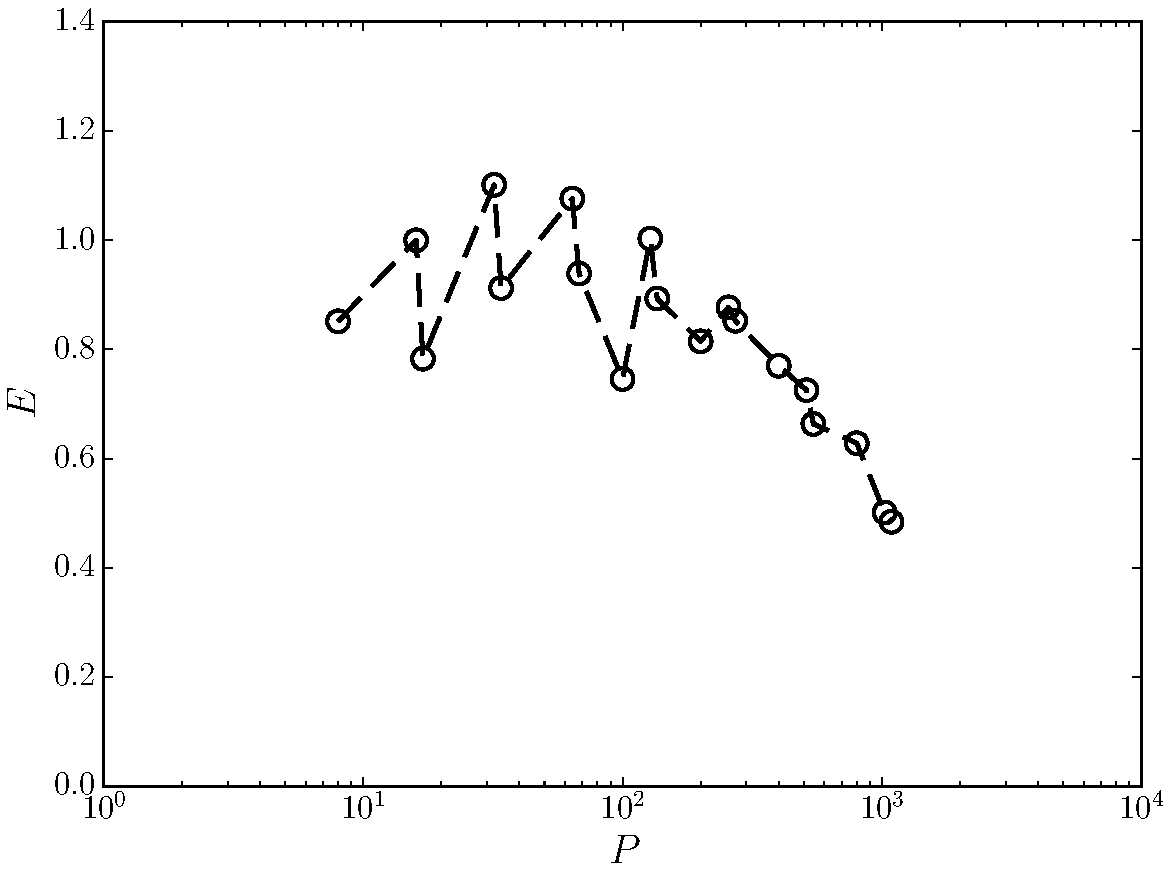
\includegraphics[width=0.5\textwidth]{Figures/strong_scaling.pdf}
\caption{\small \textit{Strong scaling performance for $N_{tot} = 256^3$ using up to 1088 cores, with a reference performance using $P_\mathit{ref} = 16$.}}
\label{fig:strong_scaling}
\end{figure}

Next, we evaluated the \textit{weak scaling} of PARTIES using a similar simulation, but with $Re_w = 200$.  The domain size and number of particles were increased in proportion to the number of processors such that the subdomain size of each processor remained constant, as shown in Table~\ref{tab:weak_scaling}.  Based on the strong scaling test, we executed the weak scaling test using $N_\mathit{tot}/P = 256^3/128$ and $N_\mathit{tot}/P = 256^3/256$, the former being the last point with perfect parallel efficiency ($\approx 100\%$) and the latter being the last point with reasonable parallel efficiency ($\approx 90\%$).

\begin{table}[t]
\centering
\begin{tabular}{c | r | r | r | r | r | r | c | c}
\hline
\hline
Run  & $N_x$ &  $N_y$ & $N_z$ & \multicolumn{1}{c |}{$N_{tot}$} & $P$ & $T(P,N_{tot})$ & $T_\mathit{write}(P,N_{tot})$ & \\
\hline
Ref   &  256 & 512 &  256 &  $33.6\times10^6$ &  256 &  76.12 &   41.25  \\
$1$   &  256 & 512 &  256 &  $33.6\times10^6$ &  512 &  43.30 &   49.13  \\
$2$   &  512 & 512 &  256 &  $67.1\times10^6$ &  512 &  79.05 &   98.99  \\
$3$   &  512 & 512 &  256 &  $67.1\times10^6$ & 1024 &  45.56 &  129.15  \\
$4$   &  512 & 512 &  512 & $134.2\times10^6$ & 1024 &  83.90 &  233.85  \\
$5$   &  512 & 512 &  512 & $134.2\times10^6$ & 2048 &  49.81 &  388.83  \\
$6$   & 1024 & 512 &  512 & $268.4\times10^6$ & 2048 & 101.84 & 1004.66  \\
\hline
\hline
\end{tabular}
\caption{\small \textit{Weak scaling configurations.  Times shown are $T(P,N_{tot})$, the time to execute 10 simulation timesteps, and $T_\mathit{write}(P,N_{tot})$, the time to write two output files.}}
\label{tab:weak_scaling}
\end{table}
Based on the strong scaling results, all simulations to be run on Stampede2 using PARTIES will be conducted with $N_{tot}/P\geq 256^3/128$. This constraint is equivalent to choosing $P$ such that each sub-domain has at least $N^3$ cells, where $N=50$. Large simulations of $N_{tot}\approx 10^9$ are expected to perform well with $P = 2048,4096$ cores for which $N = 79,63$ respectively. In the current implementation of PARTIES, writing of the 3D data structures is not parallel, but remains non-consequential to the overall performance even when outputting time resolved data. For large scale simulations, 3D data outputs will be limited to $\Delta t_{out}> 1000\Delta t$. Most of the post-processing is now done in run-time with outputs of 2D averaged data or 1D statistics, and considerable effort has recently been put into both parallelisation of the writing as well as minimization of the 3D outputs with comprehensive parallel post-processing.     

\begin{figure}[t]
\centering
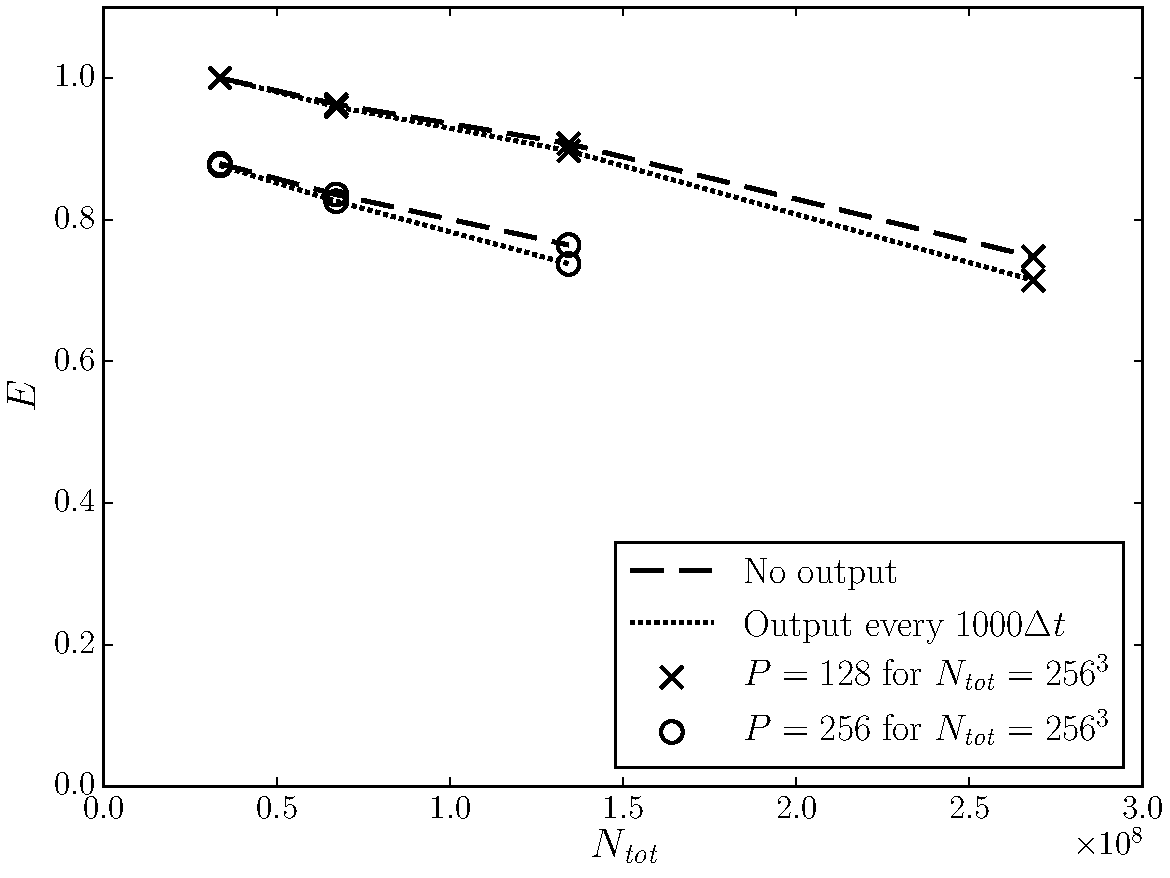
\includegraphics[width=0.5\textwidth]{Figures/weak_scaling.pdf}
\caption{\small \textit{Weak scaling performance using up to 2048 cores, with a reference performance using $P_\mathit{ref} = 128$ and $N_\mathit{ref} = 16.7\times10^6$.}}
\label{fig:weak_scaling}
\end{figure}

\begin{table}[t]
\centering
\begin{tabular}{c | r | r | r | r | r | r}
\hline
\hline
Run   & $P$       & $N_{ref} / P$        & $T(P,N_{ref})$      &  $S_{ideal}$ & $S(P,N_{ref})$    & $S / S_{ideal}$ [\%] \\
\hline
Ref   &   16      & $2097.2 \cdot 10^3$  & 39.94               &  $  1$       &  $1.00$           &  $100.0$     \\  %
$1$   &   32      & $1048.6 \cdot 10^3$  & 16.44               &  $  2$       &  $2.42$           &  $121.4$     \\  %
$2$   &   64      & $ 525.3 \cdot 10^3$  &  7.63               &  $  4$       &  $5.23$           &  $130.8$     \\  %
$3$   &  128      & $ 262.1 \cdot 10^3$  &  4.10               &  $  8$       &  $9.73$           &  $121.6$     \\  %
$4$   &  256      & $ 131.1 \cdot 10^3$  &  2.95               &  $ 16$       & $13.53$           &  $ 84.6$     \\  %
$6$   &  512      & $  66.5 \cdot 10^3$  &  1.90               &  $ 64$       & $20.96$           &  $ 65.5$     \\  %
$7$   & 1024      & $  32.8 \cdot 10^3$  &  1.31               &  $128$       & $30.42$           &  $ 47.5$     \\  %
\hline
\hline
\end{tabular}
 \caption{\small \textit{Speedup for $33.6 \cdot 10^6$ grid cells and up to 1024 cores.}}
\label{tab:speedup}
\end{table}
%
\begin{figure}[t]
\centering
\includegraphics[width=0.5\textwidth]{Figures/speedup.eps}
\caption{\small \textit{Speedup with $33.6 \cdot 10^6$ grid cells and 1604 particles.}}
\label{fig:speedup}
\end{figure}


\end{document}






